\documentclass{article}
\usepackage{iclr2026_conference,times}
\input{math_commands.tex}
\usepackage{hyperref}
\usepackage{url}
\usepackage{booktabs}
\usepackage{graphicx}

\title{Mechanism-Level Sim2Real Contracts:\\A MuJoCo Negative Result}
\author{Anonymous Authors}

\begin{document}
\maketitle

\begin{abstract}
This paper records a negative result for mechanism-level sim-to-real contracts in contact-rich manipulation.
The hypothesis was that transfer should be accepted only when explicit contact mechanisms agree between source simulation and target reality: contact onset, slip ratio, force-displacement slope, energy dissipation, and actuator lag.
We rebuilt the idea as a MuJoCo source-to-target pushing benchmark with target friction shifts, mass/compliance shifts, actuator lag, sensor bias, combined reality gaps, strong baselines, ablations, contract diagnostics, stress sweeps, and seed-level uncertainty.
The mechanism fails the submission gate.
On the combined reality gap, the proposed contract planner reaches 0.500 success, while residual adaptation reaches 0.683 and conformal filtering reaches 0.567.
Its zero false-accept rate is achieved by accepting almost no transfers.
A scalar residual ablation reaches 0.650 success, beating the full contract mechanism.
We therefore mark this project \textbf{KILL/ARCHIVE} for ICLR main.
\end{abstract}

\section{Question}
Sim-to-real transfer for manipulation is crowded with domain randomization, robust policies, system identification, residual adaptation, and causal transfer claims~\citep{prior1,prior3,prior4}.
The original bet here was narrower: instead of matching observations, a robot should transfer a simulated plan only when the physical mechanism that makes the plan work is preserved.
For pushing, such mechanisms include when contact begins, how much the object slips, how force maps to displacement, how much energy is dissipated, and how much the actuator lags.

This is an attractive story, but a submission needs more than the story.
The mechanism must improve transfer success or safety beyond strong baselines.
It must also avoid a trivial solution: reject nearly every transfer and call that safe.

\section{Benchmark}
We implement a lightweight MuJoCo source-to-target benchmark.
Each episode starts from a source simulation with nominal object mass, friction, actuator response, and contact compliance.
The target ``real'' world changes one or more mechanisms: nominal target, high friction, low friction, mass/compliance shift, actuator lag, sensor bias, and combined reality gap.
Every episode runs a source-predicted probe, a target probe, and a final target rollout.
The probe yields five contract diagnostics: onset error, slip error, force-slope error, energy error, and lag error.

We compare nine methods.
\texttt{source\_sim\_mpc} transfers the source plan.
\texttt{domain\_randomized\_mpc} plans over broad physical ranges.
\texttt{ensemble\_uncertainty\_mpc} penalizes model variance.
\texttt{system\_id\_probe\_mpc} estimates target parameters from the probe.
\texttt{residual\_adaptation\_mpc} corrects displacement using probe residuals.
\texttt{conformal\_transfer\_filter} rejects high-residual transfers.
\texttt{mechanism\_contract\_mpc} is the proposed method, using the five explicit contracts.
\texttt{oracle\_target\_mpc} has access to target parameters and is an upper bound.

\section{Main Results}
The main run uses 5 seeds, 12 episodes per seed, 7 target splits, and 9 methods, producing 3,780 MuJoCo episodes.
The ablation suite adds 420 episodes and the stress sweep adds 960 episodes.
Success means the object ends within 7.5 cm of the target.
False accept means a method accepts transfer and the final rollout fails or violates contact limits.

\begin{table}[t]
\centering
\caption{Combined reality-gap results. The contract method is safe only because it almost never accepts transfer.}
\label{tab:combined}
\begin{tabular}{lcccccc}
\toprule
Method & Succ. & 95\% CI & Error & Energy & False Acc. & Accept \\
\midrule
\texttt{random\_push} & 0.100 & 0.077 & 0.157 & 0.433 & 0.900 & 1.000 \\
\texttt{source\_sim\_mpc} & 0.517 & 0.128 & 0.094 & 0.532 & 0.483 & 1.000 \\
\texttt{domain\_randomized\_mpc} & 0.500 & 0.128 & 0.100 & 0.531 & 0.500 & 1.000 \\
\texttt{ensemble\_uncertainty\_mpc} & 0.450 & 0.127 & 0.102 & 0.514 & 0.550 & 1.000 \\
\texttt{system\_id\_probe\_mpc} & 0.500 & 0.128 & 0.091 & 0.565 & 0.500 & 1.000 \\
\texttt{residual\_adaptation\_mpc} & 0.683 & 0.119 & 0.071 & 0.531 & 0.317 & 1.000 \\
\texttt{conformal\_transfer\_filter} & 0.567 & 0.126 & 0.093 & 0.520 & 0.217 & 0.433 \\
\texttt{mechanism\_contract\_mpc} & 0.500 & 0.128 & 0.087 & 0.539 & 0.000 & 0.017 \\
\texttt{oracle\_target\_mpc} & 1.000 & 0.000 & 0.006 & 0.604 & 0.000 & 1.000 \\
\bottomrule
\end{tabular}
\end{table}

\begin{figure}[t]
\centering
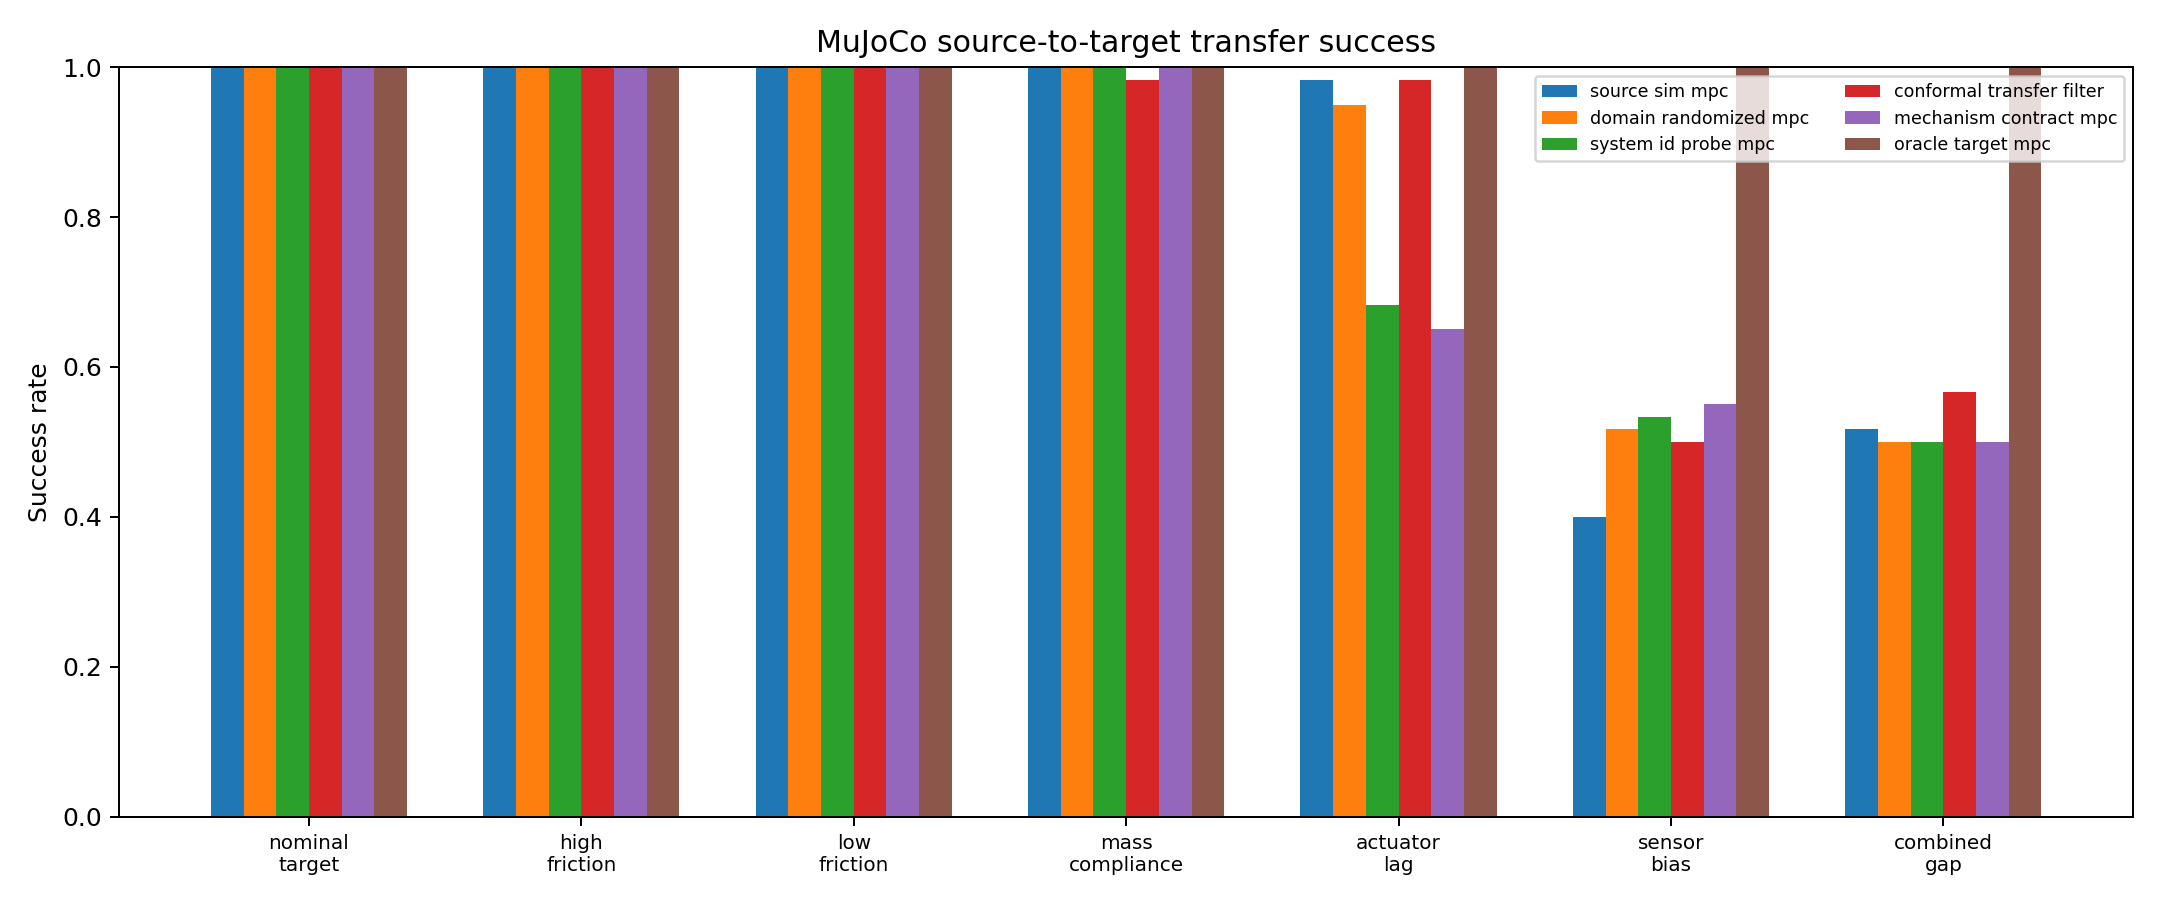
\includegraphics[width=\linewidth]{../figures/sim2real_contracts_success_by_split.png}
\caption{Transfer success across target shifts. Mechanism contracts do not dominate residual adaptation or conformal filtering.}
\label{fig:success}
\end{figure}

Table~\ref{tab:combined} is the main result.
The contract method ties or trails simple source transfer, domain randomization, and system identification, while residual adaptation is substantially better.
Pairwise seed comparisons show the contract method is below residual adaptation by 0.183 success and below conformal filtering by 0.067 success.
The contract method does have zero false accepts on the combined gap, but its accept rate is 0.017.
That is not robust transfer; it is near-total rejection.

\section{Ablations}
\begin{table}[t]
\centering
\caption{Combined-gap ablations. Scalar residuals beat the full mechanism.}
\label{tab:ablation}
\begin{tabular}{lcccc}
\toprule
Ablation & Success & 95\% CI & False Acc. & Accept \\
\midrule
\texttt{full\_mechanism\_contract\_mpc} & 0.483 & 0.128 & 0.033 & 0.033 \\
\texttt{no\_actuator\_lag\_contract} & 0.567 & 0.126 & 0.033 & 0.067 \\
\texttt{no\_contact\_onset\_contract} & 0.567 & 0.126 & 0.233 & 0.417 \\
\texttt{no\_energy\_contract} & 0.550 & 0.127 & 0.033 & 0.067 \\
\texttt{no\_force\_slope\_contract} & 0.433 & 0.126 & 0.050 & 0.083 \\
\texttt{no\_slip\_contract} & 0.600 & 0.125 & 0.017 & 0.083 \\
\texttt{scalar\_residual\_only} & 0.650 & 0.122 & 0.350 & 0.967 \\
\bottomrule
\end{tabular}
\end{table}

\begin{figure}[t]
\centering
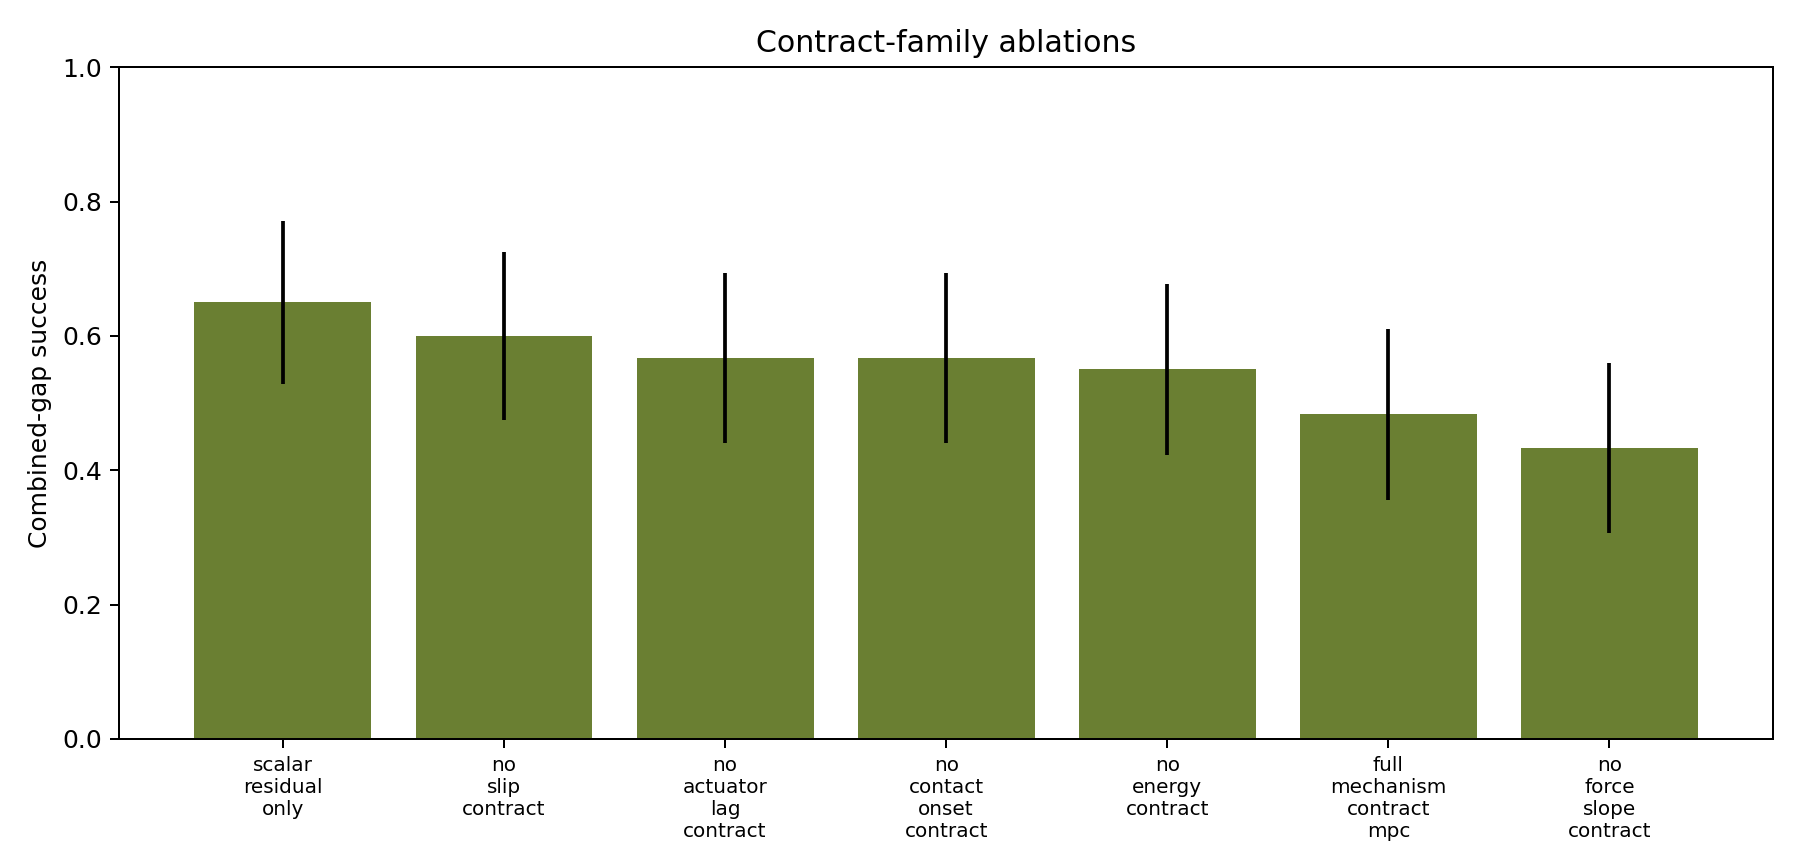
\includegraphics[width=0.85\linewidth]{../figures/sim2real_contracts_ablation_success.png}
\caption{Contract-family ablations. Several removals improve success, and scalar residuals outperform the full contract set.}
\label{fig:ablation}
\end{figure}

The ablation result is fatal for the paper thesis.
If the individual contract families were the mechanism, removing them should hurt.
Instead, removing slip, contact onset, energy, or actuator-lag contracts can improve success.
The scalar residual baseline is especially damaging: it keeps almost all transfers, reaches 0.650 success, and beats the full mechanism by 0.167 success.

\section{Contract Diagnostics and Stress Tests}
\begin{figure}[t]
\centering
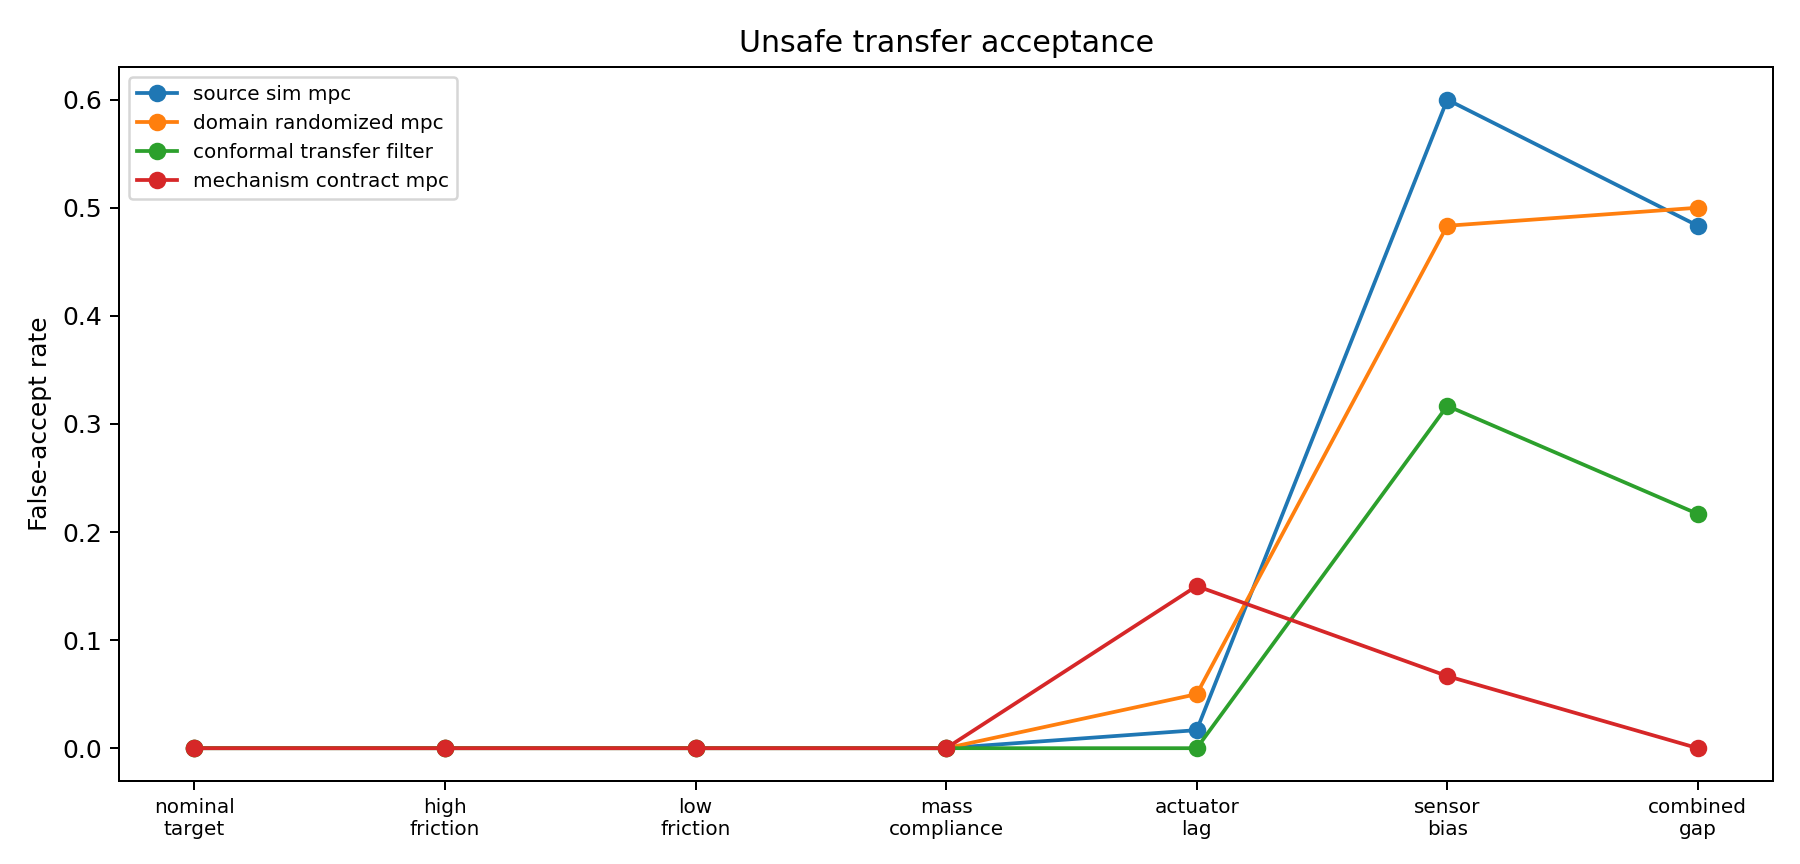
\includegraphics[width=0.82\linewidth]{../figures/sim2real_contracts_false_accepts.png}
\caption{False accepts across target shifts. Contract filtering is safe mainly because it rejects almost everything under severe shift.}
\label{fig:falseaccept}
\end{figure}

The contract scores detect synthetic contract violations by construction, but they do not reliably predict final task failure.
On the combined gap, the contract-failure correlation with rollout failure is -0.192.
On sensor bias, it is -0.482.
This means the measured contract score is not aligned with the final task metric in the way a submission claim would require.

\begin{figure}[t]
\centering
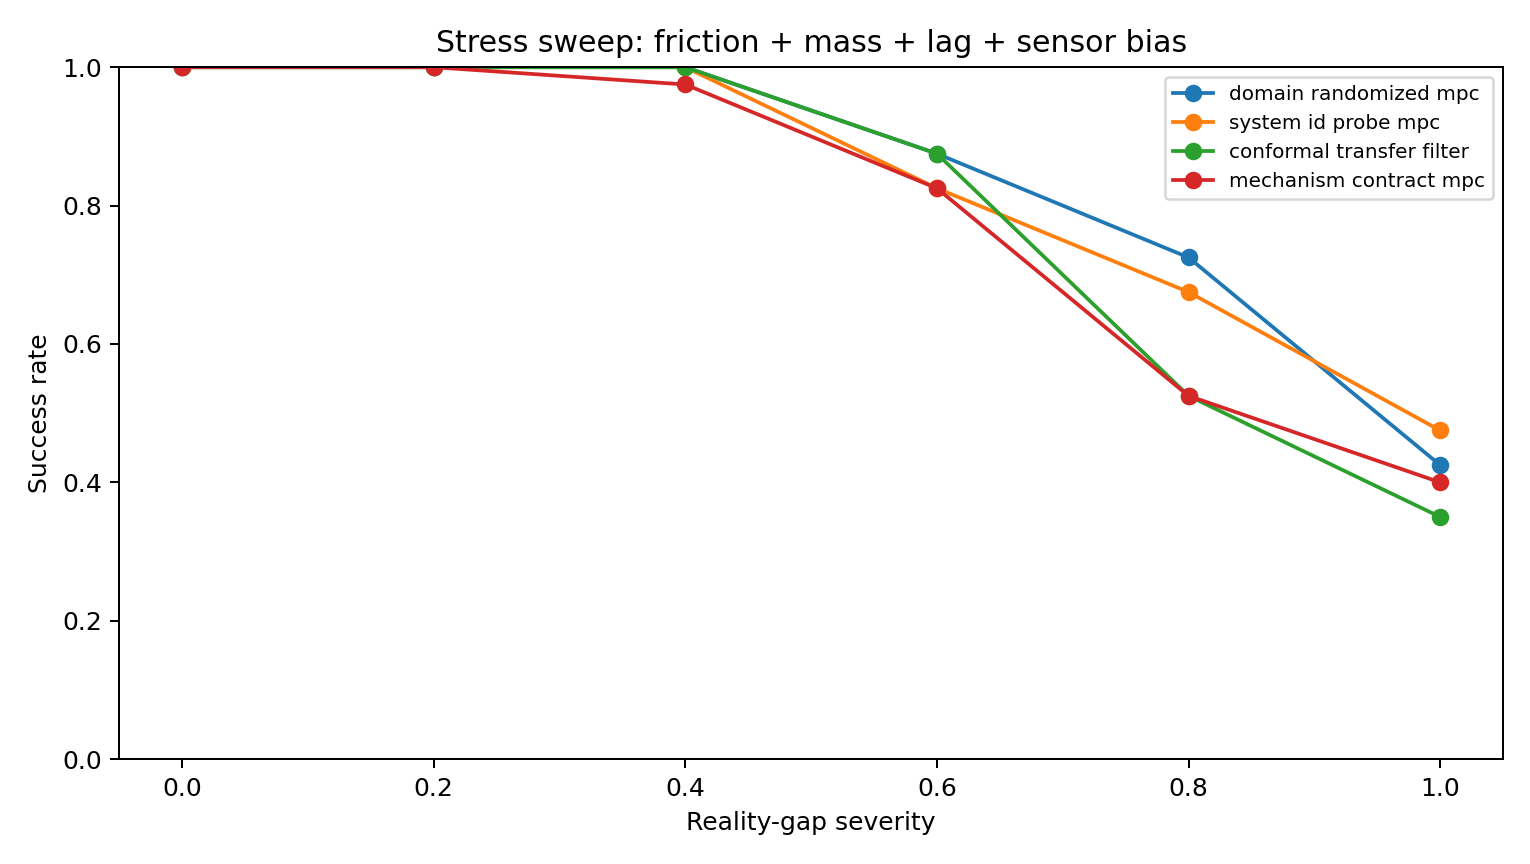
\includegraphics[width=0.82\linewidth]{../figures/sim2real_contracts_stress_sweep.png}
\caption{Stress sweep over friction, mass, actuator lag, and sensor bias. The contract method does not produce a decisive transfer curve.}
\label{fig:stress}
\end{figure}

The stress sweep further supports the archive decision.
The contract method is conservative under severe shift, but it does not establish a superior success-safety frontier over residual and conformal alternatives.

\section{Limitations}
This is a simulator-only negative result, not a hardware study.
The planners are compact analytic controllers rather than trained deep policies.
The literature audit is still local and hostile-pool based rather than a manual full-paper synthesis.
Those limitations would normally motivate a strong-revise outcome if the mechanism had shown a clear signal.
It did not.
The result should therefore be read narrowly: this implementation of mechanism-level sim-to-real contracts does not justify an ICLR-main submission.

\section{Decision}
The submission gate required explicit contracts to improve transfer success and false-accept control over domain randomization, system identification, residual adaptation, conformal filtering, and scalar residual ablations.
The evidence fails that gate.
The honest terminal action is \textbf{KILL/ARCHIVE}.
Future work should test action-conditioned contracts, richer geometry, learned residual models, and real robot or public benchmark validation before reviving the idea.

\bibliographystyle{iclr2026_conference}
\bibliography{references}

\end{document}
